\section{Le modèle SIR}
        \subsection{Histoire et amélioration}

Le modèle SIR est un modèle mathématique simple qui permet de modéliser la propagation d'une maladie infectieuse dans une population. Le modèle divise la population en trois groupes : les individus susceptibles d'être infectés (S), les individus infectés (I) et les individus guéris ou rétablies (R). Les individus passent d'un groupe à l'autre en fonction de leur état de santé. Le modèle est décrit par les équations différentielles suivantes :
	\begin{itemize}[label=$\bullet$]
	\item $$\displaystyle \frac{dS}{dt} = -\frac{\beta SI}{N}$$
	\end{itemize}
	
	\begin{itemize}[label=$\bullet$]
	\item $$\displaystyle \frac{dI}{dt} = \frac{\beta SI}{N} - \gamma I$$
	\end{itemize}
	
	\begin{itemize}[label=$\bullet$]
	\item $$\displaystyle \frac{dR}{dt} = \gamma I$$
	\end{itemize}
où S, I et R représentent respectivement le nombre de personnes dans chaque groupe, N est la taille totale de la population, $\beta$ est le taux de contact et $\gamma$ est le taux de guérison. Le modèle de Reed et Frost est un autre modèle mathématique simple qui permet de modéliser la propagation d'une maladie infectieuse dans une population. Dans ce modèle, les individus sont divisés en trois groupes : les individus susceptibles d'être infectés (S), les individus infectés (I) et les individus rétablies (R). Le modèle suppose que chaque individu infecté a une probabilité fixe de transmettre la maladie à un individu susceptible chaque semaine.
La figure \ref{fig:sir_deterministe} est un exemple de simulation du modèle SIR grâce au code python en annexe \ref{simu_det}.
	\begin{figure}[h]
    \centering
	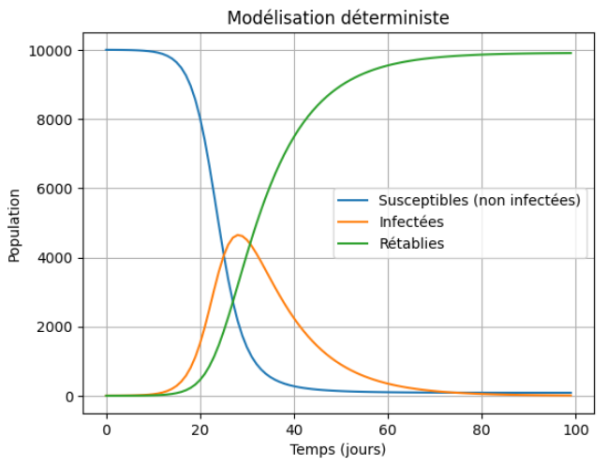
\includegraphics[width=0.5\textwidth]{figs/sir_deterministe.png}
    \caption{Évolution SIR déterministe}
    \label{fig:sir_deterministe}
	\end{figure}
	